% Copyright 2019 Clara Eleonore Pavillet

% Author: Clara Eleonore Pavillet
% Description: This is an unofficial Oxford University Beamer Template I made from scratch. Feel free to use it, modify it, share it.
% Version: 1.0

\documentclass{beamer}
\usepackage{pdfpages}
% Load Packages
\usepackage[utf8]{inputenc}
\usepackage{xcolor}
\usepackage{tikz}
\usetikzlibrary{positioning,calc}
\usepackage{graphicx}
\usepackage{hyperref}
\usepackage{amsmath}
\usepackage{listings}
\usepackage{fontawesome}
\usepackage[T2A]{fontenc}
\usepackage[utf8]{inputenc}
\usepackage[russian]{babel}

% Define Commands
\newcommand*{\ClipSep}{0.06cm} %To adjust footer logo
\newcommand{\E}{\mathrm{e}\,} %\def\I{e} % used to defined e for exp(x), see later what it should be
\newcommand{\ud}{\mathrm{d}}
\lstset{numbers=left, numberstyle=\tiny, stepnumber=1,firstnumber=1,breaklines=true,
    numbersep=5pt,language=Python,
    stringstyle=\ttfamily,
    basicstyle=\footnotesize, 
    showstringspaces=false
}

\usetheme{oxonian}
\usepackage{wrapfig}
\usepackage{listings}

\title{Използване на OpenMP. Част 2.}
\subtitle{\textit{Курс „Паралелно програмиране“}}
\titlegraphic{{
\includegraphics[width=5.3cm]{iaps.png}}} 

\author{\newline \newline Стоян Мишев}

\vspace{1cm}

\date{} %\today

\begin{document}
\lstset{language=Python}
{\setbeamertemplate{footline}{} 
\frame{\titlepage}}


\section*{План}\begin{frame}{План}\tableofcontents\end{frame}

%%%%%%%%%%%%%%%%%%%%%%%%%%%%%%%%%%%%%

\begin{frame}[plain]{Задача}

  \begin{equation}
    \int_0^1 \frac{4}{1+x^2} dx = \pi  \nonumber
  \end{equation}
\end{frame}

\begin{frame}
  \frametitle{SPMD <-> Worksharing}
  Loop

  Section

  Single

  Task
\end{frame}


\begin{frame}
  \frametitle{Loop}
  \centering
  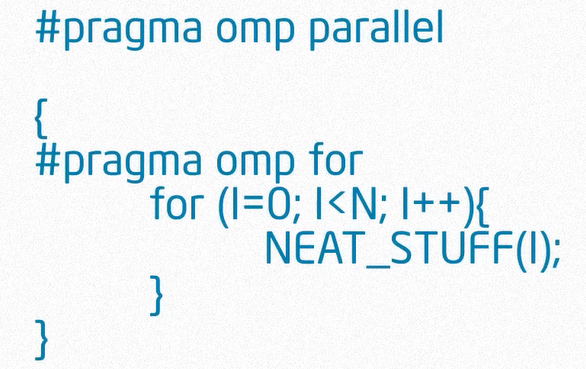
\includegraphics[width=0.5\textwidth]{for} 

  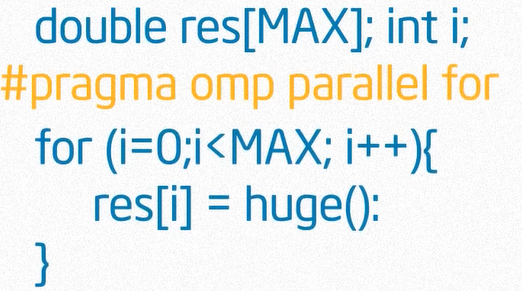
\includegraphics[width=0.4\textwidth]{for-short}
\end{frame}

\begin{frame}
  \frametitle{Schedule}
  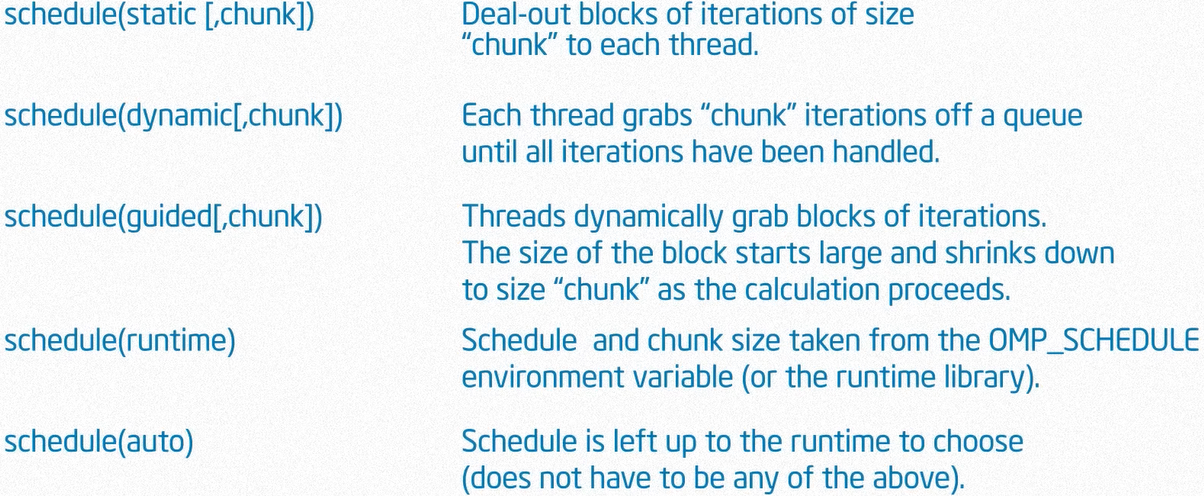
\includegraphics[width=\textwidth]{schedule}  
\end{frame}


\begin{frame}
  \frametitle{Reduction}
  \centering
  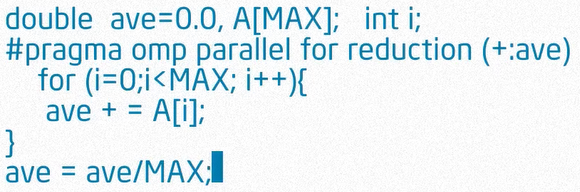
\includegraphics[width=0.8\textwidth]{reduction} \pause
  
  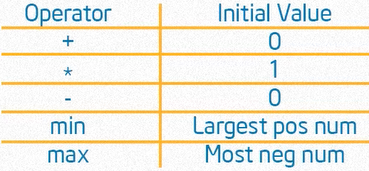
\includegraphics[width=0.6\textwidth]{reduction-init}    
\end{frame}


\begin{frame}[plain]
  \frametitle{Integral}
  \centering
  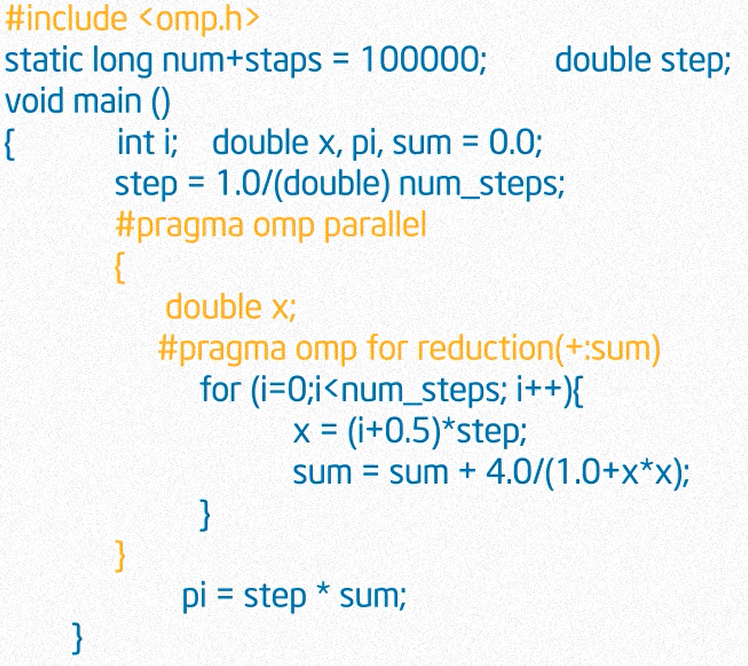
\includegraphics[width=0.6\textwidth]{integral-worksharing}\pause

  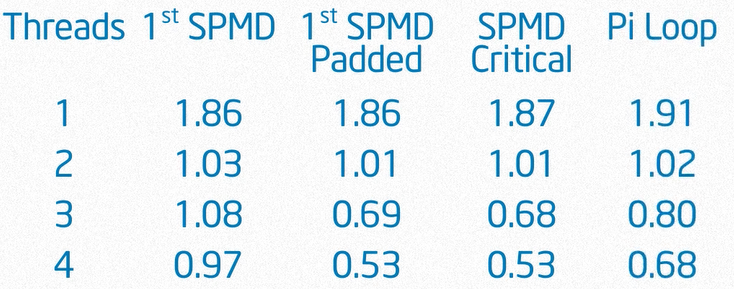
\includegraphics[width=0.55\textwidth]{integral-worksharing-time}
\end{frame}


\begin{frame}
  \frametitle{Barrier}
  \centering
  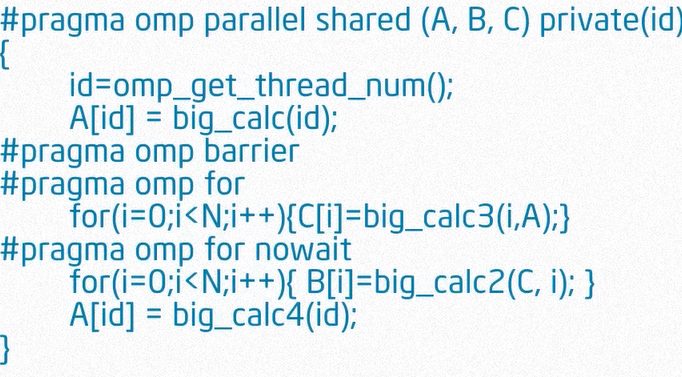
\includegraphics[width=0.7\textwidth]{barrier}
\end{frame}


\begin{frame}
  \frametitle{Master}
  \centering
  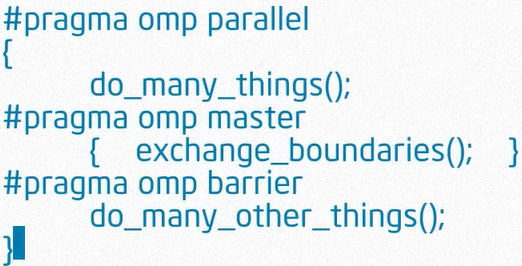
\includegraphics[width=0.7\textwidth]{master}
\end{frame}


\begin{frame}
  \frametitle{Single}
  \centering
  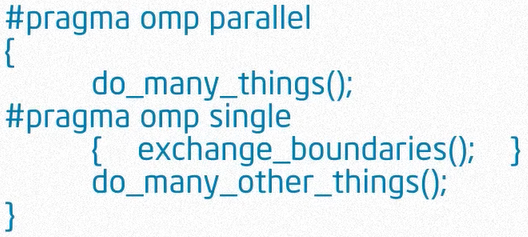
\includegraphics[width=0.7\textwidth]{single}
\end{frame}


\begin{frame}
  \frametitle{Домашна работа}
\url{https://www.youtube.com/watch?list=PLLbPZJxtMs4ZHSamRRYCtvowRS0qIwC-I}  

От ``Introduction to OpenMP 08 Discussion 3 ''
 
до ``Introduction to OpenMP 11 part 1 Module 6''.

\end{frame}



\end{document}

%%% Local Variables:
%%% mode: latex
%%% TeX-master: t
%%% End:
